\documentclass{beamer}
\usetheme{Warsaw}

\usepackage[utf8]{inputenc}
\usepackage{fancybox}
\usepackage{multimedia} 
\usepackage{subfig}
\usepackage{amsmath}
\usepackage{hyperref}
\usepackage[all]{xy}
\usepackage{algorithm}
%\usepackage{arevmath}     % For math symbols
\usepackage[noend]{algpseudocode}

\begin{document}


\title[Angewandte Mathematik] % (optional, only for long titles)
{Angewandte Mathematik
\\
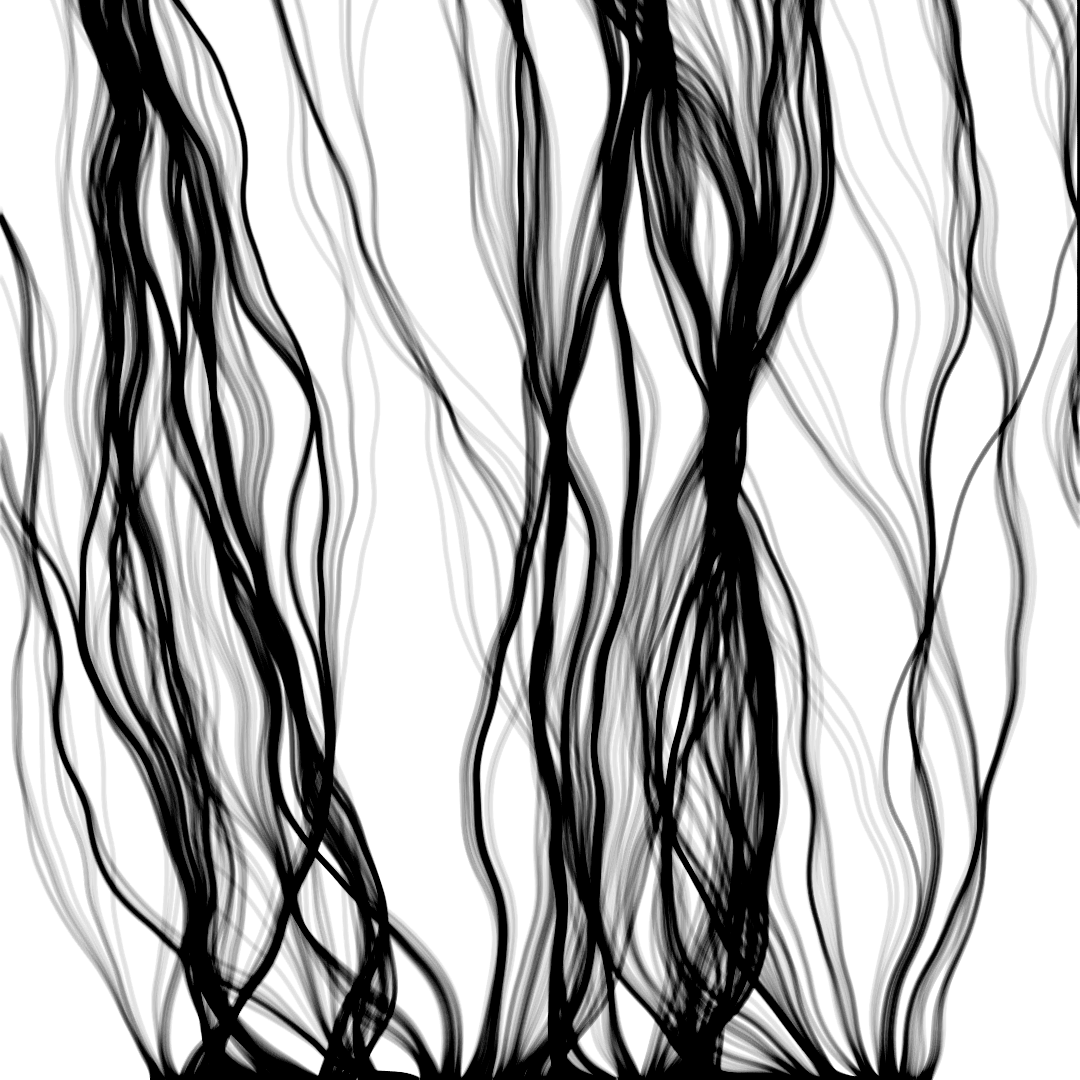
\includegraphics[scale=0.15]{images/cover}
}
\subtitle{}
\author[Dr. Johannes Riesterer] % (optional, for multiple authors)
{Dr.  rer. nat. Johannes Riesterer}

\date[KPT 2004] % (optional)
{}

\subject{Angewandte Mathematik}



\frame{\titlepage}


\begin{frame}
    \frametitle{Angewandte Mathematik}
\framesubtitle{Dynamische Systeme }
\begin{block}{Lipschitz-Stetig}
Eine  Abbildung $F : U \subset \mathbb{R} \times \mathbb{R}^n \to \mathbb{R}^n$ heißt Lipschitz-Stetig,
falls es eine Konstante $L \geq 0$ gibt  mit
$$ || F(t,x) - F(t,x') ||  \leq L || x -x' ||  $$
für alle $(t,x)$ und $(t,x')$ in $U$.
\end{block}

 \end{frame}


\begin{frame}
    \frametitle{Angewandte Mathematik}
\framesubtitle{Dynamische Systeme }
\begin{block}{Metrischer Raum}
Ein metrischer Raum $(X,d)$ ist eine Menge $X$ zusammen mit einer Abbildung $d : X \times X \to \mathbb{R}$ die linear ist in beiden Argumenten und die Dreiecksungleichung $d(x,y) \leq d(x,z) + d(z,y)$ erfüllt.  
\end{block}
\begin{block}{Beispiel}
$d(x,y) : = || y- x  ||$  wobei $||  \cdot ||$  eine Norm ist. 
\end{block}

\begin{block}{Beispiel}
Das für uns später relevante Beispiel ist der Funktionenraum mit der Maximumsnorm $|| \varphi || := \max_t | \varphi(t)|$.
\end{block}
 \end{frame}


\begin{frame}
    \frametitle{Angewandte Mathematik}
\framesubtitle{Dynamische Systeme }
\begin{block}{Banachscher Fixpunktsatz}
Es sei $(X,d)$ ein vollständiger metrischer Raum und $P: X \to X$ eine Abbildung mit $$d(P(x), P(y)) < \lambda d(x,y)$$ und $\lambda < 1$. Dann besitzt $P$ genau einen Fixpunkt $x^* \in X$ mit $P(x^*) = x^*$.

\end{block}

 \end{frame}

\begin{frame}
    \frametitle{Angewandte Mathematik}
\framesubtitle{Dynamische Systeme }
\begin{figure}[H]
      \centering
    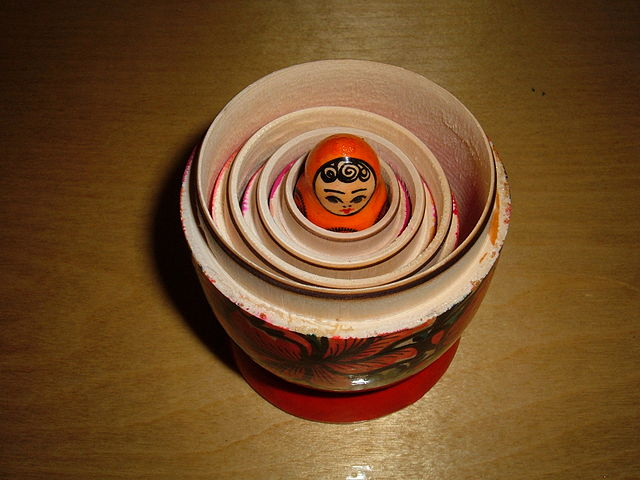
\includegraphics[width=0.7\textwidth]{images/640px-Floral_matryoshka_set_2_smallest_doll_nested.JPG}
\caption{Quelle: Wikipedia}
\end{figure}

 \end{frame}


\begin{frame}
    \frametitle{Angewandte Mathematik}
\framesubtitle{Dynamische Systeme }
\begin{figure}[H]
      \centering
    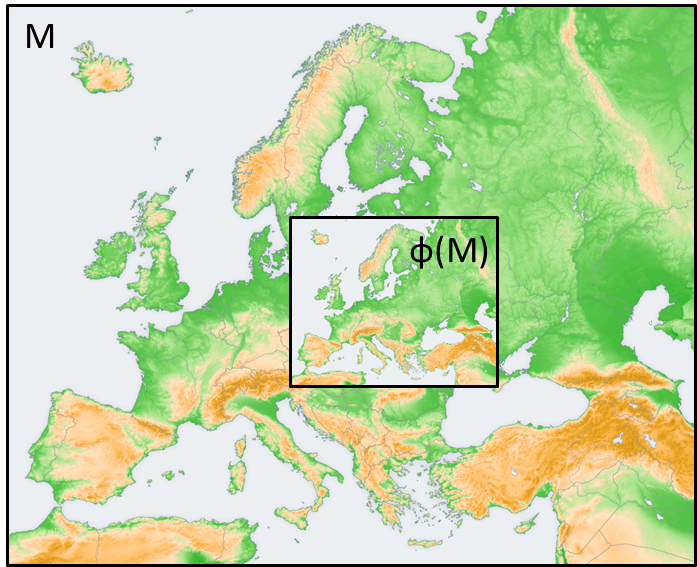
\includegraphics[width=0.7\textwidth]{images/banach}
\caption{Quelle: Wikipedia}
\end{figure}

 \end{frame}


\begin{frame}
    \frametitle{Angewandte Mathematik}
\framesubtitle{Beweis}
Wähle beliebiges $x_0 \in X$. Durch wiederholtes Abbilden erhalten wir die Folge  $x_n:= P(x_{n-1})$. Für diese Gilt nach Voraussetzung an $P$
\begin{align*}
d(x_{n+1} , x_{n}) < \lambda d(x_{n} , x_{n-1})   < \lambda^n d(x_{1} , x_{0})  \; .
\end{align*}
Mit wiederholtem Anwenden der Dreiecksungleichung gilt 
\begin{align*}
d(x_{n + m} , x_{ n}) \leq d(x_{n+1} , x_{n})  +  d(x_{n +2} , x_{n +1}) +   \cdots   +  d(x_{n + m } , x_{n +m -1}) \; .
\end{align*}
Da $\lambda < 1$ folgt $  \lim_{n \to \infty} d(x_{n + m} , x_{ n})   \leq  \lim_{n \to \infty} \frac{\lambda^n}{1 - \lambda} d(x_{1} , d_{0}) = 0$ und damit ist $x_n$ eine Cauchyfolge.  Da $(X,d)$ vollständig ist, konvergiert die Folge in $X$ gegen einen Grenzwert $x^*$. Für diesen gilt $P(x^*) =  P (  \lim_{n \to \infty}  x_n) =  \lim_{n \to \infty} P(x_n)  =  \lim_{n \to \infty} x_{n+1} = x^*$ und damit ist $x^*$ ein Fixpunkt von $P$.

 \end{frame}

\begin{frame}
    \frametitle{Angewandte Mathematik}
\framesubtitle{Dynamische Systeme }
\begin{block}{Lokaler Existenzsatz von Picard-Lindelöf}
Das dynamisches System  $$F : U \subset \mathbb{R} \times \mathbb{R}^n \to \mathbb{R}^n$$ sei lokal Lipschitz-Stetig. 
Dann gibt es zu jedem Punkt $(t_0, x_0) \in U$ ein Intervall $I_\delta (t_0) := (t_0 - \delta, t_0 + \delta) \subset \mathbb{R}$ auf dem das AWP 
$$ x' = F(t,x), \; \; x(t_0) = x_0$$
\end{block}

 \end{frame}

\begin{frame}
    \frametitle{Angewandte Mathematik}
\framesubtitle{Beweis}
Betrachte die Menge  $M: = \{ \psi : I_\delta (t_0) \to \mathbb{R}^n \; | \; ||\psi(t) - x_0 || \leq b  \}$ von Wegen in der Nähe von $x_0$ und die Abbildung
\begin{align*}
& P : M \to M \\
& (P \psi)(t) := x_0 + \int_{t_0}^{t} F(t, \psi(t)) dt
\end{align*}
Ein Fixpunkt von $P$ ist eine Lösung der Differentialgleichung. P ist eine Kontraktion.
 \end{frame}



\begin{frame}
    \frametitle{Angewandte Mathematik}
\framesubtitle{Dynamische Systeme }
\begin{block}{Lineare (gewöhnliche) Differentialgleichung.}
Eine Differentialgleichung der Form
$$ x' (t): = A(t) x(t) + b(t)$$
mit $A: I \subset \mathbb{R} \to \mathbb{R}^{n \times n}$ und $b: I \subset \mathbb{R} \to \mathbb{R}^{n}$ heißt lineare (gewöhnliche) Differentialgleichung.
\end{block}

 \end{frame}


\begin{frame}
    \frametitle{Angewandte Mathematik}
\framesubtitle{Dynamische Systeme }
\begin{block}{Existenz und Eindeutigkeit]}
Ist $x' (t): = A(t) x(t) + b(t)$ eine lineare Differentialgleichung und $A$ und $b$ stetig, so besitzt das AWP 
$$ x' (t): = A(t) x(t) + b(t) ; \; \; x(t_0) = x_0 $$
genau eine auf ganz $I$ definierte Lösung.
\end{block}
\begin{block}{Beweis}
$F(t,x):= A(t) x(t) + b(t)$ ist Lipschitz-Stetig mit Konstanten $L:= \max_{t \in J}|| A(t) ||$ für jedes kompakte Intervall $J \subset I$.
\end{block}
 \end{frame}


\begin{frame}
    \frametitle{Angewandte Mathematik}
\framesubtitle{Dynamische Systeme Systeme}
\begin{block}{Lineare (gewöhnliche) Differentialgleichung.}
\begin{itemize}
\item Die Menge $\mathcal{L}$ der auf $I$ definierten Lösungen der homogenen Gleichung $x'(t) = A(t)x(t)$ ist eine $n$-dimensionaler reeller Vektorraum.
\item $n$ Lösungen $\varphi_1, \cdots, \varphi_n : I \to \mathbb{R}^n$ bilden genau dann eine Basis für $\mathcal{L}$, wenn die Vektoren $\varphi_1(t), \cdots, \varphi_n(t)$ für ein $t \in I$ eine Basis des $\mathbb{R}^n$ bilden.
\end{itemize}
\end{block}

 \end{frame}


\begin{frame}
    \frametitle{Angewandte Mathematik}
\framesubtitle{Beweis}
Sind  $\varphi_1, \cdots, \varphi_n$ Lösungen der homogenen Gleichung, so auch $ c_1 \cdot \varphi_1 + \cdots + c_n \cdot \varphi_n$, da die Ableitung linear ist.
$\mathcal{L}$ ist somit ein Vektorraum. Definiere 
\begin{align*}
& \alpha_{t_0} : \mathcal{L} \to \mathbb{R}^n \\
& \alpha_{t_0} (\varphi) := \varphi(t_0) \; .
\end{align*} 
Aufgrund des Existenzsatzes und der linearität ist $ \alpha_{t_0}$ surjektiv und wegen der Eindeutigkeit der Lösung injektiv.
 \end{frame}


\begin{frame}
    \frametitle{Angewandte Mathematik}
\framesubtitle{Dynamische Systeme Systeme}
\begin{block}{Lineare (gewöhnliche) Differentialgleichung.}
Eine Basis  $\varphi_1, \cdots, \varphi_n$ des Lösungsraumes $\mathcal{L}$ der homogenen Gleichung $x'(t) = A(t)x(t)$ heißt Fundamentalsystem.
\end{block}

 \end{frame}

\begin{frame}
    \frametitle{Angewandte Mathematik}
\framesubtitle{Dynamische Systeme Systeme}
\begin{block}{Lineare (gewöhnliche) Differentialgleichung.}
Für eine Matrix $A \in \mathbb{R}^{n \times n}$ definiert man die Exponentialfunktion 
$$  e^{ A}  := \sum_{k= 0}^{\infty} \frac{1}{k!} A^k \; .$$
Es gilt  
$$  (e^{ tA})' = A e^{tA}  \; .$$
\end{block}

 \end{frame}

\begin{frame}
    \frametitle{Angewandte Mathematik}
\framesubtitle{Dynamische Systeme Systeme}
\begin{block}{Lineare (gewöhnliche) Differentialgleichung.}
Für eine Matrix $A$ lautet die Lösung des Anfangswertproblems $x'(t) = Ax(t)$ und $x(0) = x_0$
$$ x(t) = e^{tA} x_0 \;.$$ Ist $v_1, \cdots , v_n$ eine Basis des $\mathbb{R}^n$, so ist $e^{tA}v_1, \cdots , e^{tA}v_n$ ein Fundamentalsystem für $\mathcal{L}$. Damit bilden die Spalten von  $e^{tA}$ ein Fundamentalsystem.
\end{block}

\begin{block}{Beweis}
Es ist $x(0) = x_0$ und $x'(t)= A x(t)$. 
\end{block}
 \end{frame}


\begin{frame}
    \frametitle{Angewandte Mathematik}
\framesubtitle{Dynamische Systeme Systeme}
\begin{block}{Lineare (gewöhnliche) Differentialgleichung.}
Sei $v$ eine Eigenvektor von $A$ zum Eigenwert $\lambda$. Dann löst 
$$ \varphi_v(t) := e^{t \lambda} v$$ das AWP $x' = Ax$ mit $x(0) = v$.

\end{block}
\begin{block}{Beweis}
$\varphi_v'(t) =  \lambda  e^{t \lambda}  v =  e^{t\lambda}  \lambda v =  e^{t\lambda}  A v  = A e^{t\lambda}   v  = A  \varphi_v(t)$.

\end{block}
 \end{frame}

\begin{frame}
    \frametitle{Angewandte Mathematik}
\framesubtitle{Dynamische Systeme Systeme}
\begin{block}{Lineare (gewöhnliche) Differentialgleichung.}
Hat eine Matrix $A$ $n$ Eigenvektoren $v_1, \cdots , v_n$ zu den Eigenwerten $\lambda_1, \cdots  \lambda_n$, 
so bilden die Lösungen $ \varphi_{v_1}, \cdots  \varphi_{v_n}$ ein Fundamentalsystem.
\end{block}
\begin{block}{Beweis}
Eigenvektoren sind linear unabhängig.
\end{block}
 \end{frame}


\begin{frame}
    \frametitle{Angewandte Mathematik}
\framesubtitle{Dynamische Systeme Systeme}
\begin{block}{Hauptvektoren.}
Ein Vektor $v$ heißt Hauptvektor zum Eigenwert $\lambda$, falls es eine Zahl $s>0$ gibt mit 
$$ (A - \lambda E)^s v = 0$$
Die kleinste Zahl $s$, für die dies gilt heißt Stufe.
\end{block}

 \end{frame}


\begin{frame}
    \frametitle{Angewandte Mathematik}
\framesubtitle{Dynamische Systeme Systeme}
\begin{block}{Hauptvektoren}
Zu jeder Matrix $A \in \mathbb{R}^{n \times n}$ gibt es eine Basis aus Hauptvektoren. 
\end{block}

\begin{block}{Hauptvektoren}
    Für einen Haupvektor $v$ der Stufe $s$ zum Eigenwert $\lambda$ ist
    \begin{align*}
       e^{A t} v = e^{\lambda I t}e^{(A - \lambda I)t} = e^{\lambda t} \sum_{k=0}^{s-1} \frac{1}{k!}((A - \lambda I)^k t^k v)
    \end{align*}
\end{block}

\end{frame}


\begin{frame}
    \frametitle{Angewandte Mathematik}
\framesubtitle{Klassifikation linearer Systeme in dimension 2}
\begin{block}{Hauptvektoren}
Sei $x' = Ax$ mit $A:=\begin{pmatrix} a & b \\ c & d \end{pmatrix}$ und $\lambda, \mu$ die Eigenwerte von $A$.
Dann können folgende Fälle auftreten:
\begin{itemize}
  \item   Es gibt zwei verschiedene reelle Eigenwerte $\lambda_1, \lambda_2$. Die allgemeine Lösung lautet dann
	    $\varphi(t) = c_1 e^{\lambda_1 t} v_1 +c_2 e^{\lambda_2 t} v_2 \; c_1, c_2 \in \mathbb{R}$	mit den Eigenvektoren $v_1, v_2$.
    \item $\lambda$ ist ein doppelter reller Eigenwert.
        \begin{itemize}
            \item Der Lösungsraum $(A - \lambda I)x = 0$ hat dimension $2$. Das ist der Fall,
                wenn bis auf Basistransformation $A = \lambda I$ ist. \\
                In diesem Fall hat die Differentialgleichung die allgemeinen Lösungen 
                \begin{align*}
                    \varphi(t) = e^{\lambda t}v, \; v \in \mathbb{R}^2 \text{ beliebig}
                \end{align*}
            \end{itemize}

\end{itemize}

\end{block}

\end{frame}


\begin{frame}
    \frametitle{Angewandte Mathematik}
\framesubtitle{Klassifikation linearer Systeme in dimension 2}
\begin{block}{Hauptvektoren}
\begin{itemize}
    \item 
        \begin{itemize}
            \item  Der Lösungsraum $(A - \lambda I)x = 0$ hat dimension $1$. \\
                In diesem Fall gibt es einen Hauptvektor $h$ der Stufe $2$, also eine Lösung von 
                $(A-\lambda I)h = v$. Die allgemeinen Lösungen lauten damit
                \begin{align*}
                    \varphi(t) = e^{\lambda t} (c_1 v + c_2(h + tv)) \; c_1, c_2 \in \mathbb{R}
                \end{align*}
            \end{itemize}
    \item $A$ hat die komplex konjugierten Eigenwerte $\lambda, \bar{\lambda} \in \mathbb{C}$. Dann hat $A$ die komplexen Eigenvektoren 
            $w, \bar{w} \in \mathbb{C}^2$. Da $A$ reell ist, sind $\varphi_1(t):= Re (w e^{\lambda t})$ und 
            $\varphi_2(t):= Im (w e^{\lambda t})$. Mit $w = u + iv$ und $\lambda = \gamma + i \theta$ ergibt sich
            \begin{align*}
                \varphi_1(t) = Re (w e^{\lambda t}) = e^{\gamma t}(\cos \theta t \cdot u - \sin \theta t \cdot v) \\
                \varphi_2(t) = Im (w e^{\lambda t}) = e^{\gamma t}(\sin \theta t \cdot u + \cos \theta t \cdot v)
            \end{align*}

\end{itemize}

\end{block}

\end{frame}


\begin{frame}
    \frametitle{Angewandte Mathematik}
\framesubtitle{Klassifikation linearer Systeme in dimension 2}
\begin{block}{Hauptvektoren}
    Die Lösungen sind damit gegeben durch
            \begin{align*}
                \varphi(t) = c_1 \varphi_1(t) + c_2 \varphi_2(t)  
            \end{align*}


\end{block}

\end{frame}



 \begin{frame}
    \frametitle{Angewandte Mathematik}
\framesubtitle{Dynamische Systeme }

\begin{block}{Lösung Harmonischer Oszillator}
  
    \begin{align*}
        \begin{pmatrix}
            x_1(t) \\ x_2(t)
        \end{pmatrix} = \begin{pmatrix}
            \cos(t) & -\sin(t)  \\ \sin(t) & \cos(t)
        \end{pmatrix}   \cdot \begin{pmatrix}
            x_1\\ x_2
        \end{pmatrix}
    \end{align*}
\end{block}
\center
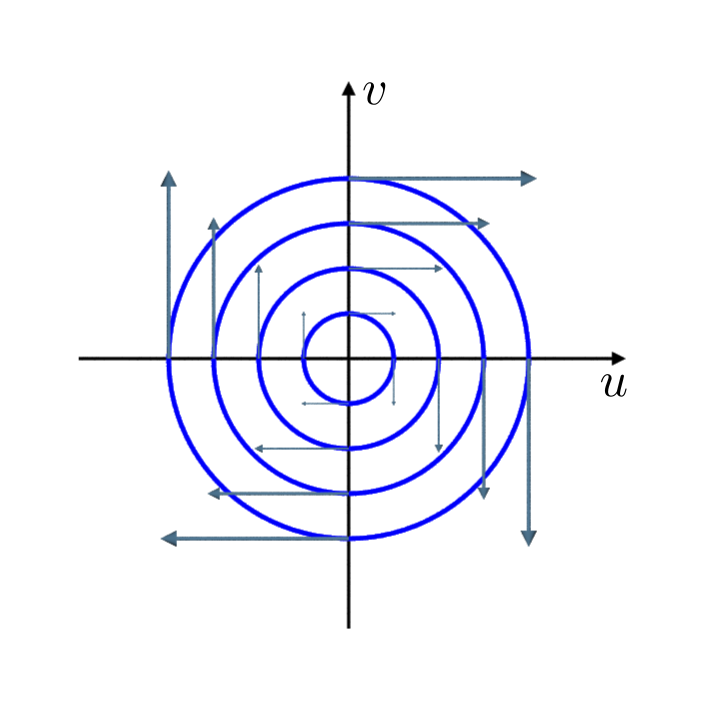
\includegraphics[scale=0.25]{images/harmonicoszillatorphasespace}
 \end{frame}



 \begin{frame}
    \frametitle{Angewandte Mathematik}
\framesubtitle{Dynamische Systeme }

\begin{block}{Harmonischer Oszillator Eigenwerte}
    \begin{align*}
    \det (\begin{pmatrix}
        0 & -1  \\ 1 & 0
    \end{pmatrix} - \lambda E) = 
    \det \begin{pmatrix}
        -\lambda & -1  \\ 1 & -\lambda  
    \end{pmatrix} = \lambda^2 +1 \Rightarrow \lambda_{1,2} = \pm i
\end{align*}
Komplexer Eigenwert.
 \end{block}
 \end{frame}


 \begin{frame}
    \frametitle{Angewandte Mathematik}
\framesubtitle{Dynamische Systeme }
\begin{block}{Lineares System mit Hauptraum}
\begin{align*}
    \frac{d}{dt}\begin{pmatrix}
        x_1(t) \\ x_2(t)
    \end{pmatrix} = 
\begin{pmatrix}
    1 & 1  \\ 1 & 0
\end{pmatrix} \cdot
\begin{pmatrix} 
    x_1(t) \\ x_2(t)
\end{pmatrix} 
\end{align*}
\end{block}

\begin{block}{Lineares System mit Hauptraum}
    \begin{align*}
    \det (\begin{pmatrix}
        1 & 1  \\ 1 & 0
    \end{pmatrix} - E) = 
    \det \begin{pmatrix}
        1-\lambda & 1  \\ 0 & 1-\lambda  
    \end{pmatrix} = (1-\lambda)^2 \Rightarrow \lambda_{1,2} = 1
\end{align*}
Doppelter Eigenwert.
\end{block}

\end{frame}

 \begin{frame}
    \frametitle{Angewandte Mathematik}
\framesubtitle{Dynamische Systeme }
\begin{block}{Eigenraum zum Eigenwert $1$}
    \begin{align*}
    \ker (\begin{pmatrix}
        1 & 1  \\ 0 & 1
    \end{pmatrix} - E) = 
    \ker \begin{pmatrix}
        0 & 1  \\ 0 & 0  
    \end{pmatrix} = \{e_1\}
\end{align*}
Doppelter Eigenwert aber Eigenraum ist eindimensional. 
 \end{block}
 \begin{block}{Hauptraum zum Eigenwert $1$}
    \begin{align*}
    \ker ( (\begin{pmatrix}
        1 & 1  \\ 0 & 1
    \end{pmatrix} - E)^2) = 
    \ker \begin{pmatrix}
        0 & 1  \\ 0 & 0  
    \end{pmatrix}^2 = \ker \begin{pmatrix}
        0 & 0  \\ 0 & 0  
    \end{pmatrix} =  \{e_1, e_2\}
\end{align*}
$e_2$ ist Hauptvektor der Stufe $2$, $e_1$ Hauptvekrot der Stufe $1$, also

$ \biggl (\begin{pmatrix}
    1 & 1  \\ 0 & 1
\end{pmatrix} - E \biggr) e_2 = e_1; \;  \biggl (\begin{pmatrix}
    1 & 1  \\ 0 & 1
\end{pmatrix} - E \biggr) e_1 = 0$ 
 \end{block}
 \end{frame}


 \begin{frame}
    \frametitle{Angewandte Mathematik}
\framesubtitle{Dynamische Systeme }

\begin{block}{Allgemeine Lösung}
    \begin{align*}
        & \varphi_1(t) := e^t \cdot e_1 = e^t \begin{pmatrix} 1 \\ 0\end{pmatrix} \\
        & \varphi_2(t) := e^t \biggl (E  +  \bigl (\begin{pmatrix} 1 & 1 \\ 0 & 1\end{pmatrix} - I\bigl)t \biggr )e_2 = e^t \begin{pmatrix} t  \\ 1 \end{pmatrix} \\
        & \varphi(t) = c_1 \varphi_1(t) +  c_2\varphi_2(t)
    \end{align*}
\end{block}
 \end{frame}


\end{document}